\documentclass{article}
\usepackage[utf8]{inputenc}

\usepackage{graphicx}
\usepackage[version=4]{mhchem}
\usepackage{siunitx}
\usepackage{glossaries}
\usepackage{xr} % For cross-referencing wit the supplemental information
\usepackage{textgreek}

\externaldocument{supplement}

% Drafting

\usepackage[latexmk]{lwarp}

\usepackage{xcolor,soul}
\usepackage{fullpage}
\usepackage{setspace}
\usepackage{blindtext}
\doublespacing

\definecolor{mwcolor}{HTML}{8af67d}
\definecolor{vgcolor}{HTML}{c88bff} % MPL purple
\definecolor{citecolor}{HTML}{c696f0} % MPL purple


% Tools for leaving todo notes around
\usepackage[colorinlistoftodos]{todonotes}
%% \renewcommand{\todo}{}
%% \renewcommand{\hl}[1]{#1}
\newcommand{\citeme}[1]{%
  \todo[color=citecolor]{%
  \ifstrempty{#1}{[citation needed]}{[cite: #1]}%
  }%
}
\newcommand{\mw}[2]{%
  \sethlcolor{mwcolor}\hl{#2}\sethlcolor{yellow}%
  \ifstrempty{#1}{}{%
    \todo[color=mwcolor]{#1 [MW]}%
  }%                  
}
\newcommand{\vg}[2]{%
  \sethlcolor{vgcolor}\hl{#2}\sethlcolor{yellow}%
  \ifstrempty{#1}{}{%
    \todo[color=vgcolor]{#1 [VG]}%
  }%                  
}

\usepackage{authblk}

\title{Origin of Rapid Delithiation In Secondary Particles Of \nca{} and \nmc{} Cathodes}

\author[1,2,3]{Mark Wolfman}
\author[1]{Brian M.\ May}
\author[4]{Vishwas Goel}
\author[4]{Sicen Du}
\author[5,6]{Young-Sang Yu}
\author[7]{Nicholas V.\ Faenza}
\author[7]{Nathalie Pereira}
\author[8]{Antonin Grenier}
\author[3]{Kamila M.\ Wiaderek}
\author[3]{Ruqing Xu}
\author[9]{Jiajun Wang}
\author[8]{Karena W.\ Chapman}
\author[7]{Glenn G. Amatucci}
\author[4]{Katsuyo Thornton}
\author[1]{Jordi Cabana\thanks{Corresponding author: jcabana@uic.edu}}

\affil[1]{Department of Chemistry, University of Illinois at Chicago}
\affil[2]{Chemical Sciences and Engineering Division, Argonne National Laboratory}
\affil[3]{X-ray Science Division, Advanced Photon Source, Argonne National Laboratory}
\affil[4]{Department of Materials Science and Engineering, University of Michigan}
\affil[5]{Department of Physics, Chungbuk National University}
\affil[6]{Advanced Light Source, Lawrence Berkeley National Laboratory}
\affil[7]{Energy Storage Research Group, Department of Materials Science and Engineering, Rutgers, The State University of New Jersey}
\affil[8]{Department of Chemistry, Stony Brook University}
\affil[9]{Harbin Institute of Technology}

\date{}

\newcommand{\nca}[1]{\ce{Li_{#1}Ni_{0.8}Co_{0.15}Al_{0.05}O_2}}
\DeclareRobustCommand{\nmc}[2][]{%
    \ifstrempty{#1}{%
        \ce{Li_{#2}Ni_{y}Mn_{z}Co_{1-y-z}O2}}{}%
    \ifstrequal{#1}{333}{%
        \ce{Li_{#2}Ni_{1/3}Mn_{1/3}Co_{1/3}O2}}{}%
    \ifstrequal{#1}{532}{%
        \ce{Li_{#2}Ni_{0.5}Mn_{0.3}Co_{0.2}O2}}{}%
}

% Techniques
\newacronym{xrd}{PXRD}{powder X-ray diffraction}
\newacronym{uxrd}{µ-XRD}{X-ray microdiffraction}
\newacronym{txm}{TXM}{transmission X-ray microscopy}
\newacronym{xas}{XAS}{X-ray absorbance spectroscopy}
\newacronym{xanes}{XANES}{X-ray absorbance near edge spectroscopy}
\newacronym{iscat}{iSCAT}{optical interferometric scattering microscopy}

% Facilities and organizations
\newacronym{ssrl}{SSRL}{Stanford Synchrotron Radiation Lightsource}

% Chemistry
%\newacronym{ecd}{ECD}{exchange current density}
\newacronym{ecd}{$i_0$}{exchange current density}
\newacronym{od}{OD}{optical depth}
\newacronym{ocv}{OCV}{open circuit voltage}

% Particles in u-XRD mapping
\newacronym{p1}{P1}{particle 1}
\newacronym{p2}{P2}{particle 2}
\newacronym{p3}{P3}{particle 3}



\begin{document}

\maketitle

%%%%%%%%%%%%%%%%%%%%%%%
\section{Introduction}
%%%%%%%%%%%%%%%%%%%%%%%



%%%%%%%%%%%%%%%%%%
\section{Results}
%%%%%%%%%%%%%%%%%%

\subsection{\Gls{uxrd} - Interparticle Dynamics}

For each particle of study, the individual 2D diffraction patterns
collected at each X-Y mapping position were integrated to 1D
patterns. The 1D patterns for each mapping position within a particle
were subsequently summed for points collected during the reaction
(Figures \ref{fig:uxrd}a,b and \ref{fig:xrd-echem}). These summations
are useful to monitor the overall evolution of diffraction peaks
during oxidation and reduction of the cathode material for each
particle observed. The diffraction patterns for all three particles in
the pristine condition match well with literature for \nca{}
\cite{Robert2015a}. There was an extra feature that varied in
intensity at Q\SI{\approx3.6}{\per\angstrom}, representative of
metallic \ce{Li} (PDF \#00-001-1131). Small extraneous peaks occurred
due to random aberrations in individual pixels on the diffraction
detector.

The diffraction peaks for \gls{p1} began to shift at the onset of
oxidation (Figure \ref{fig:uxrd}a). The shifts observed in \gls{p1}
were consistent with similar observations of \emph{operando} XRD of
the ensemble average, as opposed to individual particles in \nca{}
electrodes, in prior work \cite{Robert2015, Grenier2017}. \gls{p2}
(\ref{fig:xrd-echem}b) also had a change in XRD peak positions during
cycling. While the peak positions of the extreme states (pristine,
charged, discharged) were consistent with those of \gls{p1}, the peaks
did not begin shifting until the cell was at a potential of
\SI{\approx4.5}{\volt}. Both \gls{p1} and \gls{p2} discharged at
approximately the same rate. \gls{p3} (\ref{fig:xrd-echem}c) had no
apparent change in diffraction peak positions during charge or
discharge. This may have been due to poor connection to the carbon and
binder of the electrode.

Consideration of individual peaks provides more detailed structural
information. The (003) reflection had an initial decrease in $Q$
(Figure \ref{fig:uxrd}a), corresponding to an expansion of the $c$
axis of the structure of the oxide, which represents the stacking of
the alternating transition metal and lithium layers. It was followed
by a sudden opposite shift beyond the initial position, indicating
shrinkage of the lattice along the same direction, while still during
delithiation. This trend has been reported before. The initial
expansion is attributed to electrostatic repulsion by the \ce{O^{2-}}
ions when \ce{Li+} ions are initially removed between consecutive
layers \cite{Robert2015}. In turn, the subsequent collapse is driven
by steric effects, and reflect the complete removal of \ce{Li+} ions,
which act as pillars of the layered framework. The (104) diffraction
peak gradually shifted to higher $Q$, or lower $d$, upon removal of
\ce{Li} from the material (Figure \ref{fig:uxrd}b). This shift
reflects the balance between the trend along $c$ and the continuous
decrease in the $a$ dimension. In this case, the decrease was
attributed to the shortening of metal oxygen distances due to the
oxidation of the transition metal ions (mainly \ce{Ni}), which
decreased their ionic radius.

Unit cell parameters for each diffraction pattern were extracted
through Le Bail refinements and plotted as a function of cell
potential for \gls{p1} and \gls{p2} (Figures \ref{fig:uxrd}d and
\ref{fig:cell-pars}). The unit cell parameters reflected the trends
observed in the diffractograms presented in Figures \ref{fig:uxrd}a,b
and \ref{fig:xrd-echem}, as well as measurements of the ensemble
average of an electrode available in the literature
\cite{Robert2015a}. The cell parameters for \gls{p1} (\ref{fig:uxrd}d)
began shifting at a cell potential between
\SIrange{3.0}{3.8}{\volt}. The precise value is unknown as the
temporal resolution of the experiment was insufficient to capture a
full map during the rapid increase in potential at the beginning of
the charge. The unit cell parameters for \gls{p2} began shifting at
\SI{\approx4.5}{\volt}, consistent with the peak shifts in
\ref{fig:xrd-echem}b. These results led to the qualitative conclusion
that the rates of delithiation of each individual particle were
different and not uniquely represented by the electrochemical response
collected for the whole electrode.

\subsection{u-XRD - Rates of (De)lithiation}

Comparison of the \gls{xrd} patterns and unit cell parameters for
individual particles during the first cycle demonstrated differences
in rates of reaction. By estimating the amount of \ce{Li} present in
the material at different points during the cathode oxidation, we can
quantify the rate of delithiation. The \ce{Li} content can be directly
related to the unit cell parameters of \gls{p1} and \gls{p2} at
different points in time, by correlating them with \gls{xrd}
measurements of the ensemble average of a \nca{} electrode during
galvanostatic cycling from Robert et al\cite{Robert2015}. In this
reference study, \nca{} was cycled twice with a cutoff potential of
\SI{4.8}{\volt} and the cell parameters were associated to the average
\ce{Li} content in the material calculated from the specific capacity,
or charge passed, of the cell (i.e., coulometrically). During the
first cycle, the overall \nca{} electrode underwent a heterogeneous
transformation driven by kinetic limitations due to the presence of
\ce{Li2CO3}, which is electronically insulating, on the particle
surfaces. \ce{Li2CO3} is oxidized to \ce{CO2} during this first
oxidation. As a result, in the second cycle, the electrode transformed
via the expected pathways of a solid solution. We compared our data to
the second cycle from the work by Robert et al., since we did not see
any evidence of heterogeneous behavior in either the electrochemistry
or XRD patterns of individual particles (\ref{fig:xrd-echem}). In
order to directly compare trends in \ce{Li} content, the experimental
unit cell parameters were shifted so that the unit cell parameters for
the pristine state were equal to first value for the second charge of
the reference data, which accounts for scalar discrepancies in the
measurement.

\todo{Update the following text with $\frac{t}{t_c}$.}

Figure \ref{fig:uxrd}e shows how the \ce{Li} content within \nca{}
changed as a function of time during the charge-discharge cycle,
calculated by measuring the variation in \ce{Li} content extracted
from the measured change in \emph{c} parameter. Similar trends were
observed when calculating \ce{Li} content using the \emph{a}
parameter. For both \gls{p1} and \gls{p2} (\ref{fig:uxrd}e) the rate
of delithiation was initially slow, followed by a sudden
increase\todo{make this more precise re: negative rates}. In the case
of \gls{p1}, the delithiation during the first \SI{\approx3}{\hour}
proceeded at \SI{\approx0.025}{\ce{Li}\per\hour}, or C/40, followed by
a deceleration until \SI{\approx9}{\hour} passed. After this period,
the overall content of the particle was
\ce{Li_{0.88}Ni_{0.80}Co_{0.15}Al_{0.05}O2}. At this point, the
reaction dramatically accelerated nearly 10-fold from the initial
rate, to \SI{\approx0.3}{\ce{Li}\per\hour}, or C/3.33 until an average
composition \nca{0.53} where the rate decelerated again until the sign
of the current was reverted. In the case of \gls{p2} there was very
little delithiation for the first \SI{\approx27}{\hour} of the charge
of the cell. Delithiation proceeded down to an average content of
\nca{0.92} at \SI{\approx0.03}{\ce{Li}\per\hour}, or C/33, followed by
a 20-fold increase in rate, to \SI{\approx0.66}{\ce{Li}\per\hour}, or
C/1.5. When an average composition \nca{0.53} was again reached, the
reaction slowed down, running below 0.1 \ce{Li}/h, or C/10, for the
remainder of the oxidation. Particles relithiated rapidly during cell
discharge, with no periods of slow activity. The states that were
captured (negative values for \emph{Li removed/hour}) showed faster
rates of relithiation earlier in the discharge for both \gls{p1} and
\gls{p2}, reflecting the fastest rates at intermediate contents of
\ce{Li} in \nca{x}, qualitatively consistent with the oxidation.

\gls{p1} and \gls{p2} both achieved the same level of delithiation at
the end of the charge sequence, observed in Figure \ref{fig:uxrd}e and
by the peak positions in Figures \ref{fig:uxrd}a,b and
\ref{fig:ind-peaks}. Since \gls{p2} did not start delithiating until
late in the charge sequence, its maximum rate of delithiation was more
than double that of \gls{p1}. This observation has no precedent in the
literature for reactions involving solid solutions, where homogeneity
removes the activation barrier toward nucleation of two-phase
mechanisms. It is particularly intriguing considering that the whole
electrode was discharged at a low constant current. It can be
hypothesized that it is due to subtle variations in overpotential
between particles as a result of a different connectivity with the
electrical circuit through the carbon additive (electrons) and the
pores that contain electrolyte (ions). Particle size may have also had
an impact. Since \gls{p2} was approximately half the size of \gls{p1},
the \ce{Li} diffusion lengths out of the particle would have been
shorter. Neither of these explanations is satisfactory to predict the
change in rate for an individual particle. It is worth noting that the
changes happen at approximately similar \ce{Li} contents for both
particles studied, suggesting that the oxidation of the material
changes its physical properties, such as electronic and ionic
conductivity. Follow-up experiments are needed to evaluate this
point. Both particles relithiated to \nca{x}, where $x$ was between
\numrange{0.88}{0.97}.

\subsection{TXM - \nmc{}}

\subsubsection{\nmc[333]{} Inter-particle Dynamics}

Dilute (20\%) \nmc[333]{} electrodes were assembled in modified
coin-cells, and operando \gls{txm} \gls{xas} frame-sets were collected
during the first galvanostatic charge/discharge cycle (Figure
\ref{fig:txm-nmc}). Localized \gls{xas} K-edge spectra were produced
from operando \gls{txm} frame-sets and then averaged over individual
particles. Example \gls{txm} frames showing several particles in a
field of view are shown in Figure \ref{fig:OD-frames}. Upon
delithiation, a progressive increase was seen in the energy of the
absorption edge and the associated whiteline (Figures
\ref{fig:isobestic-point} and \ref{fig:kedges}). Comparison of the
\ce{Ni} near-edge structure at increasing degrees of delithiation
revealed an isobestic point at \SI{8351}{eV} (Figure
\ref{fig:isobestic-point}a), often associated with the co-existence of
two spectroscopic signals with varying contributions to the observed
spectrum. Ideally, chemically pure reference samples are prepared for
the two constituents and the observed spectra analyzed by linear
combination fitting of the two reference spectra, as is done for
\ce{LiFePO4}\cite{wanli2016}. However, the absence of a miscibility
gap for layered cathodes prevents the preparation of chemically pure
reference samples. Instead, a more direct approach is used. Figure
\ref{fig:isobestic-point}b shows spectral mixing of the two extremes
from Figure \ref{fig:isobestic-point}a in ratios ranging from 0 to
1. Since the whiteline peak is broad relative to the energy difference
between the two components, the maximum of the linear combinations
changes smoothly over the full range of spectral mixing (Figure
\ref{fig:isobestic-point}c). This allows the whiteline position to be
used directly as an approximation of \ce{Ni} oxidation. Instead of
simply selecting the energy with maximum optical depth for a given
pixel, the full spectrum at each \gls{txm} pixel was fit with a
combination of a background line, arctangent function, and Gaussian
peak (\ref{eq:kedge-fitting} and Figure
\ref{fig:kedge-decomposition}), after which the whiteline energy was
extracted from the fit parameters. In addition to providing a
precision beyond the energy resolution of the instrument, this
approach was more tolerant of noise in individual micrographs since
the fitting routine relied on the entire spectrum as input.

\todo{Update this text to use $\frac{t}{t_c}$.}

\todo{We'll probably re-write portions of this to be for NCA, instead
  of NMC.}

\todo{Update this text to indicate that the NMC-333 is showing second
  charge.}

Fields of view containing multiple secondary particles were selected
from within the coin-cell window (Figure \ref{fig:txm-nmc}a), allowing
comparison of the dynamics between separate particles. Since different
layered materials have different starting \ce{Ni} oxidation states and
therefore different whiteline positions (Table
\ref{tab:bulk-xas-extraction} and Figure
\ref{fig:bulk-xas-extraction}), whiteline energies were compared to
the lowest value observed for any particle in the field of view during
the operando experiment, reported here as \textDelta{}whiteline. The
mean energies for several \nmc[333]{} secondary particles are shown in
Figure \ref{fig:nmc-particles}a,b. Initially, the whiteline energies
were constant, indicating no \ce{Ni} oxidation. After
\SI{\approx10}{\hour}, the whiteline energy increased rapidly by
\SI{\approx3.75}{eV} over a period of \SI{5}{\hour}. Five out of the
six particles underwent this rapid oxidation simultaneously, while the
remaining particle transitioned within the next \SI{2}{\hour}. Over
the remaining \SI{15}{\hour} of the charge cycle, the particle
whiteline positions increased gradually by an additional
\SI{0.6}{eV}. This particle-level behavior is in contrast with the
that seen by in-situ ensemble-average \gls{xas}\cite{deb2005}, which
shows a gradual increase in whiteline position over the full range of
delithiation (Table \ref{tab:bulk-xas-extraction} and Figure
\ref{fig:bulk-xas-extraction}a). The total change in whiteline energy
for all observed secondary particles was \SI{>4}{eV} (Figure
\ref{fig:txm-nmc}d). While ensemble \gls{xas}
studies\cite{deb2005,muto2009} did not reach the \SI{4.7}{V} cell
cut-off potential needed for full lithium extraction and hence full
\ce{Ni} oxidation, extrapolation of the trend in Table
\ref{tab:bulk-xas-extraction} and Figure
\ref{fig:bulk-xas-extraction}a predicts a change in whiteline energy
upon full delithiation of \SI{\approx3}{eV}. This discrepancy between
particle-level and ensemble average \ce{Ni} oxidation suggests that an
appreciable portion of the particles in the specimens measured by
ensemble \gls{xas} had not reached their fully oxidized states. During
discharge (Figure \ref{fig:nmc-particles}a), the particles' whitelines
gradually moved to lower energies, indicating gradual reduction of
\ce{Ni}. The whiteline energy did not return to the pristine starting
point, demonstrating that the particles did not reach fully reduced
\ce{Ni} when discharged to \SI{3.3}{V}.

A second experiment was conducted during the first charge cycle, but
optimized for time resolution (Figure \ref{fig:txm-nmc}d). The
same initial latent phase and subsequent rapid oxidation were seen,
however individual particles underwent the rapid oxidation
asynchronously over the \SI{5}{\hour} window (Figure
\ref{fig:nmc-particles}c). Once rapid oxidation had occurred, the
subsequent gradual increase to \SI{4.1}{eV} was again observed. In
both experiments, the peak in the rate of change of the potential
($\dedt$, Figure \ref{fig:echem-derivatives}a,b) occurred once all
particles had undergone that rapid transition in oxidation state
(Figure \ref{fig:nmc-particles}a,c).

\begin{table}
  \begin{tabular}{c c c | c c c}
    \multicolumn{3}{c|}{\nmc[333]{x}} & \multicolumn{3}{c}{\nca{x}} \\
    x & Whiteline /eV & \textDelta{} /eV & x & Whiteline /eV & \textDelta{} /eV \\
    \hline\hline
    0.945 & 8353.98 & 0.21 & 1.00 & 8348.84 & 0.00 \\
    0.751 & 8354.72 & 0.94 & 0.80 & 8349.61 & 0.78 \\
    0.570 & 8355.45 & 1.68 & 0.60 & 8350.14 & 1.30 \\
    0.386 & 8356.12 & 2.35 & 0.25 & 8350.78 & 1.95 \\
    0.257 & 8356.43 & 2.66 & 0.00 & 8351.16 & 2.32 \\
  \end{tabular}
  \caption{Reported energies of \ce{Ni} K-edge whiteline. In-situ
    \gls{xas} of \nmc[333]{} (Ref. \cite{deb2005}) and ex-situ
    \gls{xas} \nca{} (Ref. \cite{muto2009}). Data extracted from
    published figures using
    WebPlotDigitizer\cite{webplotdigitizer}. Relative shifts in
    whiteline energy (\textDelta{}) calculated as difference from
    fully lithiated state (x=1).}
  \label{tab:bulk-xas-extraction}
\end{table}

\subsubsection{\nmc[532]{}}

Operando \gls{txm} \gls{xas} was also performed using a dilute
(\SI{20}{\percent}) \nmc[532]{} cathode in a modified coin-cell
(Figure \ref{fig:txm-nmc}e). The galvanostatic charge profile (Figure
\ref{fig:nmc532-particles}) showed the expected initial slow change in
potential, followed by a slight increase in the rate of change of
potential after \SI{12}{\hour}, similar to \nmc[333]{} (Figure
\ref{fig:nmc-particles}b,d). However, the \nmc[532]{} cathode showed
almost no initial peak in cell potential at \SI{2}{\hour}, as was
observed for \nmc[333]{} cathodes. During the first half of the charge
cycle, particles again exhibited an initial latent phase followed by
rapid increase in whiteline energy (Figure \ref{fig:txm-nmc}c,e),
consistent with the particle-level dynamics observed in \nmc[333]{}
(Figure \ref{fig:txm-nmc}b,d). X-ray micrographs were not collected
beyond \SI{10.5}{\hour} due to scheduled facility maintenance, and so
the values calculated for $\frac{t}{t_c}$ in Figure \ref{fig:txm-nmc}e
should not be considered as a measure of the time to complete a full
charge, but rather the time fraction of the actual charge applied. All
but one particle had entered this rapid transition before the last
operando \gls{txm} frame-set was collected and the increase in the
rate of change of potential at \SI{12}{\hour} (Figure
\ref{fig:echem-derivatives}f).



%%%%%%%%%%%%%%%%%%%%%
\section{Discussion}
%%%%%%%%%%%%%%%%%%%%%

%%%%%%%%%%%%%%%%%%%%%%%%%%%%%%%%
\section{Materials and Methods}
%%%%%%%%%%%%%%%%%%%%%%%%%%%%%%%%

\subsection{\gls{uxrd} Mapping}

The \nca{} composite electrode tape was cast in a dry room (dew point
of \SI{<-35}{\celsius}) using the Bellcore method
\cite{Tarascon1996}. A mixture of \nca{}, poly(vinylidene
fluoride-co-hexafluoropropylene) (PVDF-HFP, Kynar 2801, Elf Atochem),
carbon black (Super P, MMM), propylene carbonate (Aldrich), and
acetone (Aldrich) was used for the casting slurry. After casting, the
tape was allowed to dry in air, and then the propylene carbonate
plasticizer was extracted by soaking the tape in 99.8\% anhydrous
diethyl ether (Aldrich). The electrode tape had a mass composition of
\SI{20}{\percent} active material, \SI{20}{\percent} carbon additive,
and \SI{60}{\percent} binder. Prior to storage in the Ar-filled
glovebox, the tape was dried under vacuum at \SI{120}{\celsius}
overnight.

The AMPIX electrochemical cell was utilized to allow X-ray penetration
through the electrode \cite{borkiewicz2012}. Lithium metal was used as
the counter electrode and the electrolyte was composed of 1M
\ce{LiPF6} in a 1:1 mixture of ethylene carbonate:dimethyl
carbonate. Glass fiber served as the separator.

Diffraction maps were collected at the microprobe beamline at sector
34 at the Advanced Photon Source (APS), Argonne National Laboratory
(ANL). An incoming monochromatic beam at \SI{25}{\kilo\electronvolt}
(\SI{0.4959}{\angstrom}) with a size of approximately 0.5 x
\SI{0.5}{\micro\meter} was shone through the AMPIX cell onto the
sample. The intensity of the diffracted beam was collected in
transmission geometry by a MAR165 CCD detector, with 4096 x 4096
pixels, each measuring \SI{40}{\square\micro\meter}, used in 2 x 2
binning mode.

Particle locations were determined through absorption contrast imaging
over the \ce{Ni K_\alpha} emission line at
\SI{\approx8}{\kilo\electronvolt}. Once particles were located, the
sample was moved relative to the beam using a step size of
\SI{1}{\micro\meter} and an exposure time of
\SI{10}{\second}. Two-dimensional diffraction maps were collected in
this manner continuously over the charge-discharge cycle. At each
exposure, or mapping position, a single full 2D diffraction pattern,
averaging over the depth of the material, was collected (an example is
seen in \ref{fig:2Ddiffraction}). After one map was collected for each
particle, a positive current was applied so that the charge rate would
be c/20 (in which removal of a full \ce{Li} equivalent would complete
in \SI{20}{\hour}). The cut-off potential for the cell was set for
\SI{4.8}{\volt}, to ensure a complete oxidation of the \nca{}. After
holding the cell near \SI{4.8}{\volt} for several hours, the cell was
discharged at a negative current equal in magnitude to that of the
charge. The data was collected using EPICS channel-access data
acquisition and control software.

The 2D diffraction data collected by the beamline was integrated using
the FIT2D software package developed by ESRF \cite{Hammersley1996,
  Hammersley1997}. The integrated data was processed with the Scimap
analysis package \cite{Wolfman2015}, in which the determination of the
peak position yielded a set of unit cell parameters for each mapping
position, which were plotted using Python. An ensemble diffraction
pattern for each particle at each state of charge was obtained by
summing the patterns at each mapping position. These patterns
underwent batch Le Bail refinement by the TOPAS software developed by
Bruker to produce plots of unit cell as a function of charge-discharge
for each particle as a whole.

\subsection{TXM - \nca{}}

\todo{Get materials and methods from Young-Sang}

\subsection{TXM - \nmc{}}

\nca{} (NAT-1050), \nmc[333]{} (NM-3100) and \nmc[532]{} (NCM-045T)
were purchased from TODA America, Inc.\ and either stored under
ambient atmosphere (Figures \ref{fig:isobestic-point},
\ref{fig:nca-discharge-features}, \ref{fig:nca-line-scan},
\ref{fig:nca-irradiation}, \ref{fig:nmc532-particles},
\ref{fig:nmc532-maps}, \ref{fig:echem-derivatives}a-d) or in a dry
room followed by an argon-filled glovebox (Figures
\ref{fig:nmc-particles}, \ref{fig:nmc-maps},
\ref{fig:echem-derivatives}e,f, \ref{fig:nca-particles},
\ref{fig:kedge-decomposition}). \nca{} or \nmc{} powder
(\SI{20}{\percent}, TODA) and acetylene black (\SI{60}{\percent}) were
ground in a mortar and pestle, then mixed with polyvinylidene fluoride
(Solvay, \SI{2}{\percent} in N-methyl-2-pyrrolidone) to equal
\SI{20}{\percent} of dry composite. The resulting slurry was spread
onto battery grade aluminum foil using a cylindrical applicator set to
\SI{102}{\micro\meter} coating thickness. Electrode laminate was dried
in ambient atmosphere under infrared lamp for \SI{\approx15}{\min} and
placed in vacuum oven at \SI{110}{\celsius} overnight.

Cells for operando \gls{txm} were prepared by drilling holes of
\SI{800}{\micro\meter} (bottom, cathode-side), \SI{1500}{\micro\meter}
(top), or \SI{3000}{\micro\meter} (spacer, anode-side) diameter in the
centers of the corresponding coin-cell parts (2032, 316L stainless
steel, Hohsen Corp.). \SI{12.7}{\milli\meter} diameters cathodes were
assembled in these modified coin-cell parts with \SI{1}{M} \ce{LiPF6}
in 1:1 EC/DMC electrolyte and \SI{12.7}{\milli\meter} diameter \ce{Li}
metal anode inside an argon-filled glovebox. Once crimped, holes in
coin-cell were covered with \SI{1}{\micro\meter} thick \ce{Si3N4}
windows (Norcada NX5200F) using Torr-Seal vacuum-rated
epoxy. Assembled and sealed cells were removed from the glovebox and
mounted in the X-ray microscope.

\gls{txm} was performed at either the Stanford Synchrotron Radiation
Lightsource beamline 6-2c (Figures \ref{fig:nca-particles},
\ref{fig:nca-discharge-features} and \ref{fig:nca-line-scan}) or the
Advanced Photon Source beamline 8-BM-B (Figures
\ref{fig:nmc-particles}, \ref{fig:nmc-maps},
\ref{fig:nmc-maps-discharge}, \ref{fig:nca-irradiation},
\ref{fig:nmc532-particles}, and \ref{fig:nmc532-maps}), both equipped
with an XRadia transmission microscope. Beamline 6-2c utilizes a
56-pole, 0.9-Tesla Wiggler with 1.2 mrad acceptance focused and
\num{\approx1e-4} energy resolution ($\frac{\Delta E}{E}$). A
\SI{60}{nm} outer-zone-width objective zone-plate was used to render a
magnified image on a $2048 \times 2048$ charge-coupled device with
binning factor 2, producing $1024 \times 1024$ intensity
images. Beamline 8-BM-B utilizes a bending magnet source. The
remaining optical setup is similar to beamline 6-2c.

Operando data acquisition was performed by collecting frames at each
energy of both the specimen and a reference frame with no cell or
sample in the field of view. Image processing was performed using the
xanespy package\cite{xanespy}. Optical depth (OD) images were
calculated from the object frame ($I$) and reference frame ($I_0$) as
$$OD = \log{\big(\frac{I_0}{I}\big)}$$ All images within a full
operando experiment were aligned using multiple passes (as needed) of
the \texttt{register\_translation} function provided by
scikit-image\cite{walt2014} using the mean optical-depth frame as the
target image. Image normalization was performed on each frame by
subtracting the median optical depth of all background pixels
(determined by thresholding using Otsu's method\cite{otsu1979}) of
that frame\cite{jin2015}. Pixels not containing an appreciable level
of \ce{Ni} spectral signal were masked by calculating the ratio of the
edge jump (difference between the post-edge and pre-edge optical
depths) to the standard deviation of the optical depth spectrum. This
ratio was calculated for the whole frame-set, then a threshold for the
mask was determined using Otsu's method\cite{otsu1979} through
scikit-image\cite{walt2014}. Spectra for pixels passing this edge
filter were then fit with a linear combination of a background line,
Gaussian peak and arctangent function:

\begin{equation}
  OD(E) = t + s\bigg[\frac{1}{\pi}\arctan(\sigma (E-E_0)) + \frac{1}{2} +
    a\mathrm{e}^{\frac{-(E-E_0-b)^2}{2c^2}} + m(E-E_0)\bigg]
  \label{eq:kedge-fitting}
\end{equation}

with fitting parameters $\sigma$ to control the width of the
arctangent edge jump; $a, b, c$ to control the height, position and
width of the Gaussian whiteline peak; $m$ to control the slope of the
background; $E_0$ to represent the absolute energy of the edge; and
$s, t$ to control the overall scale and vertical offset of the
spectrum. Fitting was performed with the
\texttt{scipy.optimize.leastsq} wrapper around the MINPACK
\texttt{lmdif} routine\cite{scipy}. Whiteline positions were extracted
by re-sampling the above parametric function with 200 energies and
selecting the energy of maximum optical depth. Plotting was performed
using matplotlib\cite{matplotlib}.



%%%%%%%%%%%%%%%%%%%%%
\section{Conclusion}
%%%%%%%%%%%%%%%%%%%%%

%%%%%%%%%%%%%%%%%%%
\section*{Figures}
%%%%%%%%%%%%%%%%%%%

\begin{figure}
  \includegraphics{figures/NCA_xrd.png}
  \caption{Operando \gls{uxrd} of \nca{} secondary particle
    agglomerates during first charge. \todo{Write a more detailed
      caption.}}
  \label{fig:uxrd}
\end{figure}

\begin{figure}
  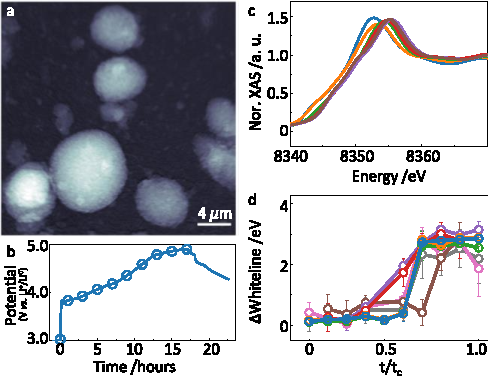
\includegraphics{figures/nca_txm.pdf}
  \caption{Operando \gls{txm} of \nca{} during first charge. (a) Mean
    optical depth frame of \nca{} particles. (b) Applied potential to
    operando cell during galvanostatic charging at \todo{what current,
      mA/g}. (c) Normalized spectra from \emph{ex-situ}
    ensemble-average \gls{xas}. (d) State-of-charge determined by
    whiteline position relative to overall state of charge in (c) for
    individual particles of \nca{}. Error bars represent one standard
    deviation over pixels within the given particle.}
  \label{fig:txm-nca}
\end{figure}

\begin{figure}
  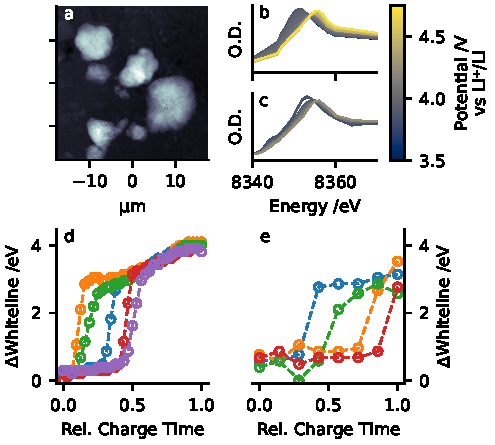
\includegraphics{figures/nmc_txm.pdf}
  \caption{Operando \gls{txm} of \nmc[333]{} and \nmc[532]{} during
    first charge. (a) Mean optical depth frame of \nmc[333]{}
    particles. (b,c) Median optical depth spectra of active material
    during (b) second charge of \nmc[333]{} and (c) first charge of
    \nmc[532]{}. (d,e) Changes in median whiteline energies relative
    to start of charging for individual particles of (d) \nmc[333]{}
    during second charge and (e) \nmc[532]{} during first charge.}
  \label{fig:txm-nmc}
\end{figure}


\end{document}
